\documentclass[prb,preprint]{revtex4-1} 
% The line above defines the type of LaTeX document.
% Note that AJP uses the same style as Phys. Rev. B (prb).

% The % character begins a comment, which continues to the end of the line.

\usepackage{amsmath}  % needed for \tfrac, \bmatrix, etc.
\usepackage{amsfonts} % needed for bold Greek, Fraktur, and blackboard bold
\usepackage{graphicx} % needed for figures
\usepackage{epstopdf}


\begin{document}

% Be sure to use the \title, \author, \affiliation, and \abstract macros
% to format your title page.  Don't use lower-level macros to  manually
% adjust the fonts and centering.

\title{Could a more precise measurement of the gravitational constant lead to Planckian SI units?}
% In a long title you can use \\ to force a line break at a certain location.

\author{Michael Ebersold}
\email{michael.ebersold@uzh.ch} 
% If there were a second author at the same address, we would put another 
% \author{} statement here.  Don't combine multiple authors in a single
% \author statement.
\author{Prasenjit Saha}
\email{psaha@physik.uzh.ch}
% Please provide a full mailing address here.
\affiliation{Physik-Institut, University of Zurich, Winterthurerstrasse 190, 8057 Zurich, Switzerland}

% See the REVTeX documentation for more examples of author and affiliation lists.

\date{\today}

\begin{abstract}
We present a new idea how the gravitational constant could be measured more precisely and if it could lead to a true Planckian basis for the SI unit system of measurement.
\end{abstract}
% AJP requires an abstract for all regular article submissions.
% Abstracts are optional for submissions to the "Notes and Discussions" section.

\maketitle % title page is now complete


\section{Introduction} % Section titles are automatically converted to all-caps.
% Section numbering is automatic.

In the late 19th century, Max Planck was working on reports about the irreversible process of radiation. He worked out a new entropy law to explain the empirical Wien law of radiation. This required him to introduce two new physical constants, which nowadays are known as the Planck constant and the Boltzmann constant \cite{Tomilin1999}. As a consequence, he described in 1899 a unit system which is based on fundamental natural constants only and thus free of anthropocentric arbitrariness. He pointed out the advantage of such a system in the following words:\cite{Planck99}\\

\begin{quote} ...ihre Bedeutung f\"{u}r alle Zeiten und f\"{u}r alle, auch au{\ss}erirdische und au{\ss}ermenschliche Kulturen notwendig behalten und welche daher als  ``nat\"{u}rliche Ma{\ss}einheiten" bezeichnet werden k\"{o}nnen... \end{quote}

\begin{quote} ...These necessarily retain their meaning for all times and for all civilizations, even extraterrestrial and non-human ones, and can therefore be designated as ``natural units"... \end{quote}

Planck units are defined in such a way that five universal physical constants are given by a numerical value of 1 when expressed in these units. Today the five constants are the speed of light in vacuum $c$, the gravitational constant $G$, the reduced Planck constant $\hbar$, the Boltzmann constant $k_B$ and the Coulomb constant $\left(4 \pi \epsilon_0\right)^{-1}$. Planck had defined them in a somewhat different form and did not adopt any electromagnetic unit. But the natural extension is to include the Coulomb constant, another possibility is to use the elementary charge $e$ to define a basic unit of charge \cite{Tomilin99}.\\
These constants can each be linked with a fundamental theory in physics that is widely accepted and universal: $\hbar$ with quantum mechanics, $c$ with special relativity, $G$ with general relativity, $k_B$ with thermodynamics and statistical mechanics, and $e$ or $\left(4 \pi \epsilon_0\right)^{-1}$ with electrodynamics.\\


The International System of Units (SI) is the commonly used system of measurement. Its beginnings go back to the French Revolution in 1799 as a precursor of the metric system was implemented. With the signing of the Convention of the Metre in 1875, new international prototypes of the metre and the kilogram were established. In the early twentieth century electromagnetic units joined the system and it underwent constant improvement, until in 1960 the modern form, called the Système International d'Unités (SI), was launched. Since the Mole joined the system of measurement in 1971, the SI unit system is in its present form.\\

To come away from the definitions based on artefacts, specific physical states and idealized experiments and because it is technologically possible to measure physical constants to high accuracy, the International Committee for Weights and Measures (CIPM) has proposed new definitions of the SI base units, which likely will be adopted in fall 2018 at the next General Conference on Weights and Measures. The revision of the SI unit system in 2018 goes towards a Planckian based system, since the values of seven physical constants get fixed and thereby define the seven base units. 
To get a truly Planckian, hence ``most natural", basis for the SI, one would have to exchange the ground state hyperfine splitting frequency of the caesium-133 atom $\Delta \nu_{\mathrm{Cs}}$ with the gravitational constant $G$ and then define the second by  
\begin{equation}
\mathrm{s} = \sqrt{\frac{h \, G}{c^5}}.
\end{equation}

\begin{equation}
\begin{aligned}
\mathrm{kg} &= 1.832\ldots \times 10^7
               \left(\frac{G}{hc}\right)^{\!1/2} \\
\mathrm{m}  &= 2.468\ldots \times 10^{34}
               \left(\frac{c^3}{hG}\right)^{\!1/2} \\
\mathrm{s}  &= 7.399\ldots \times 10^{42}
               \left(\frac{c^5}{hG}\right)^{\!1/2} \\
\mathrm{K}  &= 2.015\ldots \times 10^{-33}
               \left(\frac{Gk^2}{hc^5}\right)^{\!1/2}
\end{aligned}
\end{equation}


Because these four natural constants would have fixed numerical values, this definition is exact. Such a definition would lead to an SI system that is based on fundamental natural constants and therefore stable over time and realizable everywhere. Also completely new and more precise measurements could be designed without having to revise the definitions of the units \cite{Fischer16}. The big problem is, that the uncertainty in the measurements of $G$ is very large large. In Fig.~\ref{fig:Gmeasurements} the latest and most precise measurements of the gravitational constant are plotted together with the recommended CODATA value and its uncertainty. At first glance one notices, that the measured values are not even in good agreement with each other.\\

The big problem that this approach faces, is that the current definition of the second which is based on the hyperfine splitting frequency in the Caesium 33 atom, is much more accurate. \\  





\begin{figure}
	\centering
	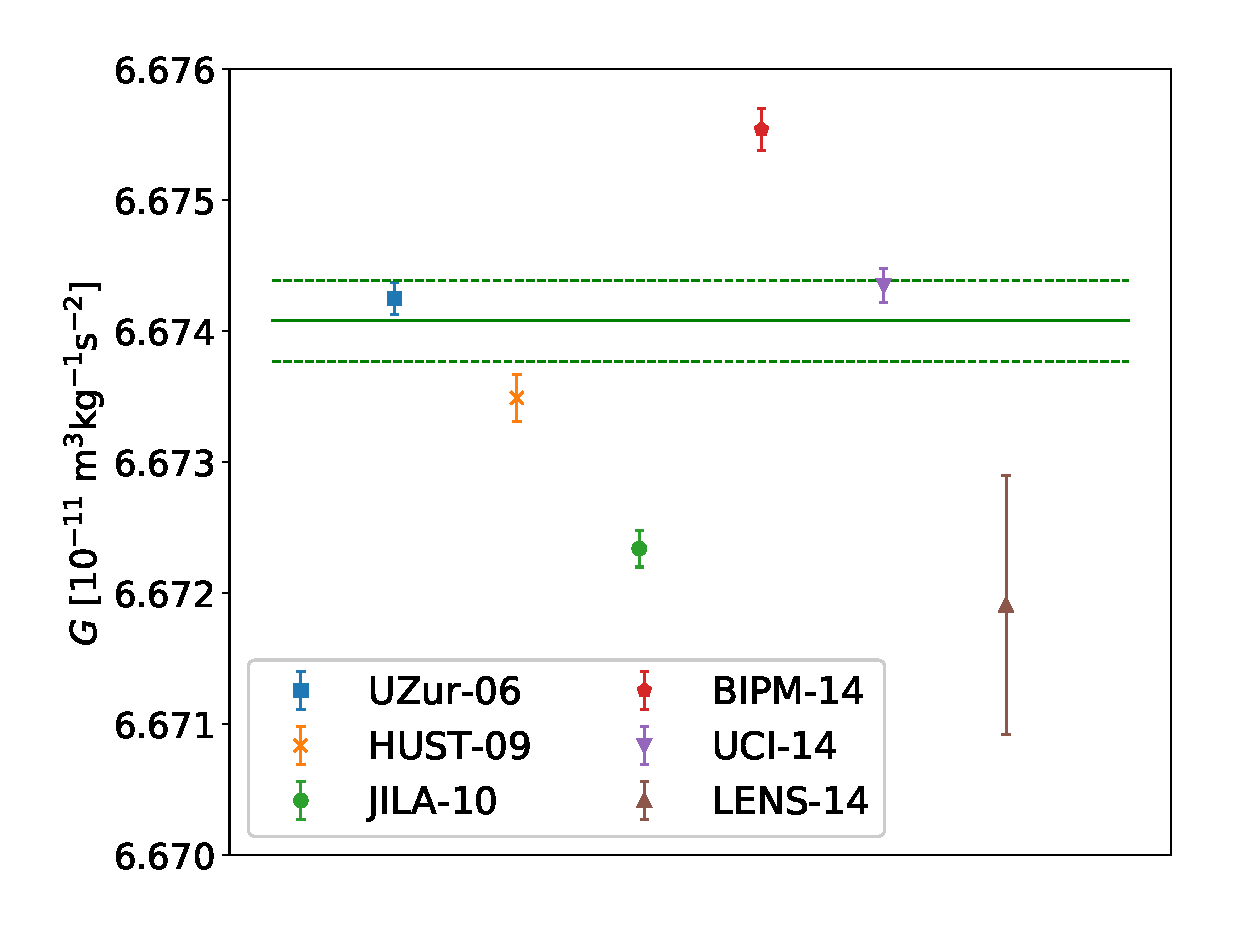
\includegraphics[width=\textwidth]{img/plotGmeas}
	\caption{The data points represent six of the most recent measurement of the gravitational constant. The green line represents the recommended CODATA value and its uncertainty.}
	\label{fig:Gmeasurements}
\end{figure}

\section{A new approach to measure $G$}

The measurements of the gravitational constant sketched in Fig.~\ref{fig:Gmeasurements} have all been done by measuring the very small force with a mechanical apparatus, expect the one with cold atom interferometry. However, it is difficult to exactly measure the weak gravitational force and it is doubtful if there will be significant improvements in measurement uncertainty with this techniques. Also the disagreement of current measurements suggests a demand for new, potentially different measurements. \\

\subsection{Description of new measurement}
Newton's law of gravitation does not only explain why an apple falls down from a tree, it also explains orbits. So if one has two bodies of masses $m_1$ and $m_2$, on which the only force acting is their respective gravitational attraction, they will orbit around their common barycenter. This orbit is described by Kepler's laws. The third law, given in Eq.~(\ref{eq:kepler3}), states that the square of the orbital period $P$ is directly proportional to the cube of the semimajor axis $a$ of the orbit. In this proportionality factor, the gravitational constant $G$ appears. To get a feeling what the dimensions of such an experiment could be, choose for example lead balls with a diameter of about 10 cm, their mass then is about 6 kg. If one then chooses a semimajor axis of 15 cm, the orbital period would be roughly 3.5 hours and the gravitational force acting between the two bodies is of order $10^{-8}$ N. In Fig.~\ref{fig:sketch} we show a sketch on how this would look like.
\begin{figure}
	\centering
	\includegraphics[width=0.9\textwidth]{img/sketchnonumb.pdf}
	\caption{Sketch on how the two masses inside the cavity of a spacecraft orbit around each other.}
	\label{fig:sketch}
\end{figure}
\begin{equation}\label{eq:kepler3}
P^2 = \frac{4 \, \pi^2}{G(m_1+m_2)}a^3
\end{equation}
If one measures the position of the two masses very accurately, it is possible to deduce the gravitational constant. The main difference to other techniques is that position measurements can be very accurate compared to directly measuring the gravitational force.\\

So the goal is to have a two-body system which is freely falling. The only way to achieve this over some time, is to go to space. Thus, one has to design a spacecraft with a cavity that contains the two masses and a position measurement apparatus. The spacecraft is then put in space, preferably to a Lagrange point of the earth-sun system, in order to prevent large inertial forces. To get an improvement in the precision of the gravitational constant, the positions of the two balls have to be known very accurately. Best suitable would probably be a laser interferometry system, which can yield precisions down to some nanometers.\cite{Loughridge13} \\

This approach appears simple, but it brings various difficulties with it. It is practically impossible to have a clean system, where only the respective gravitational force is acting between the two bodies, so one has find out what effects could possibly disturb the system and then either make them as small as possible or correct for them. \\

\subsection{Disturbing effects}

\textbf{Radiation pressure:} In space, there is a constant bombardment of radiation and charged particles from the sun, the so called solar wind. Thus the envelope of the cavity has to protect the two balls. Since the activity of the sun and the direction of the solar wind varies much, the spacecraft must be able to correct its position around the freely falling masses inside the cavity.\\
Furthermore, there is thermal radiation inside the cavity, that could disturb the orbit. To estimate the force on a ball exerted by radiation, we use the Stefan-Boltzmann law. The radiation pressure $p_r$ can be written as a third of the energy density of the electromagnetic radiation. With fundamental thermodynamics one can relate the radiation pressure to the temperature $T$
\begin{equation}
\label{Stefan-Boltzmann}
p_r = \frac{1}{3} u = \frac{1}{3} a T^4
\end{equation}
where the constant $a$ follows from Planck's radiation law and is
\begin{equation}
\label{eq:a}
a = \frac{8 \pi^5 {k_\mathrm{B}}^4}{15 c^3 h^3}.
\end{equation}
We have now a direct relation between radiation pressure and the temperature in the cavity. Then we can estimate the force exerted on a ball of radius $r$ by just multiplying the pressure with the area
\begin{equation}
F = \frac{1}{3} \pi r^2 a T^4.
\end{equation}
As we can see, this force is highly temperature dependent. In order to minimize this influence, one should deploy a temperature as small as possible in the cavity. In fact, if a cooling system based on liquid helium is installed, temperature can be brought down to about 4 K. Such a low temperature results in a radiation pressure of about $10^{-14} \, \mathrm{N} \, \mathrm{m}^{-2}$, which leads to a force on the balls in the order of $10^{-16}$ N. Compared to the gravitational force, this is orders of magnitude less and thus we don't have to worry about effects of radiation pressure.\\

\textbf{Influence of the position measurement:} In general, one has to pay attention as soon as one undertakes a measurement on a physical system, because every measurement can disturb the system. In this case we have a laser that measures the position of two masses which are in an orbit but the photons from the laser exerts an additional force on the masses. To give a rough estimation of this influence, we can compare the radiation pressure of the laser with the one of thermal radiation in the cavity, which we estimated before. In terms of the power $P$ of the laser and the area of the balls $A$, the radiation pressure is
\begin{equation}
\label{eq:radpress}
p_r = \frac{P}{c\,A}.
\end{equation}
On behalf of minimizing the impact of the position measurement, a laser with small power should be used. If we assume a laser with a power of 1 mW, the radiation pressure is in the order of $10^{-10} \, \mathrm{N} \, \mathrm{m}^{-2}$. This is a factor of $10^4$ more than radiation pressure of thermal radiation in the cavity, but the laser doesn't have to shoot photons on the balls constantly. Only for the actual measurement a short pulse has to be sent. If this pulse has a duration of less than roughly $0.1$ ms, its disturbing effect on the orbit is in the same range as the effect of thermal radiation and is thus negligible too.\\

\textbf{Coulomb force:}
Since the electromagnetic force is orders of magnitude stronger than the gravitational force, the balls must be absolutely neutral. A possible source of charges are cosmic rays or the solar wind, so they have to be protected as good as possible. If we want that the Coulomb force between the balls is in the order of $10^{-16} \,\mathrm{N}$ or smaller, and thus negligible, the maximal allowed charge on the balls is about $6 \cdot 10^{-14}\,\mathrm{C}$, which corresponds to roughly $4 \cdot 10^5$ elementary charges.\\

\textbf{Coriolis effect}
\label{sec:coriolis}
The Coriolis force is a fictitious force which only acts on moving bodies in a rotating reference frame. If we imagine the spacecraft located stationary at a Lagrange point of the earth-sun system, it is situated in a rotating frame around the earth-sun barycenter. With respect to this frame, the balls are on their orbit in movement. Thus, there will be a Coriolis acceleration
\begin{equation}
\label{eq:coriolis}
\ddot{\vec{r}}_\mathrm{c} = - 2 \; \vec{\omega} \times \dot{\vec{r}}.
\end{equation}
Here $\vec{\omega}$ is the angular velocity vector of the rotating frame and $\dot{\vec{r}}$ is the velocity vector in the two-body system. Since we don't know the exact orientation of our system with respect to the earth-sun orbital plane, we will have to fit for it.\\

\textbf{Centrifugal and tidal forces}
\label{sec:tidal}
The two masses in the spacecraft should be in a free fall and only feel their respective gravitational attraction. But this is not possible to achieve for both masses simultaneously.\\
Since we are in a non-inertial, rotating frame, there is a centrifugal force. The centrifugal acceleration $\ddot{\vec{r}}_{\mathrm{Z}}$ is proportional to the distance vector $\vec{r}$ and scales with $\omega^2$, where $\omega$ is the angular velocity of the sun-earth reference frame:
\begin{equation}
\label{eq:centrifugalacc}
\ddot{\vec{r}}_{\mathrm{Z}} = \vec{\omega} \times \left( \vec{\omega} \times \vec{r} \right) 
\end{equation}
On the other hand, there are tidal forces. Imagine if one mass is closer to the sun-earth barycenter, the gravitational force on it is slightly bigger than on the other mass. This results in a correction proportional to the distance too. One can approximate the tidal acceleration as
\begin{equation}
\label{eq:tidalacc}
\ddot{\vec{r}}_{\mathrm{\tau}} \approx \frac{2 \, G \, M_\odot}{R^3} \, \vec{r}.
\end{equation}
In this equation $M_\odot$ is the solar mass and $R$ is the radius of the orbit around the sun. With Kepler's third law one can rewrite the tidal acceleration as a function of the orbital period squared of the sun-earth reference frame. Thus it scales the same way as the centrifugal force. The effect is off course tiny, since the system under consideration is much smaller compared to the earth-sun system. To estimate the magnitude of the centrifugal and tidal acceleration relative to the gravitational acceleration between the two balls, we find that their ratio is proportional to the orbital periods squared
\begin{equation}\label{a_ratio}
\frac{\ddot{r}_{\mathrm{\tau}}}{\ddot{r}_\mathrm{G}} \propto \frac{P^2}{{P_\odot}^2} \approx 10^{-7},
\end{equation}
here $P_\odot$ corresponds to one year, whereas $P$ is the orbital period of the two balls. So tidal and centrifugal effects are about $10^{-7}$ times smaller than the respective gravity of the two balls.
In choosing the reference frame such that the net force in the system barycenter is zero, we can correct with a term in the equations of motion for the two-body system, which is proportional to the distance. Because we are in a 3-dimensional space, and possibly the influences of the different axis could mix, we have to multiply the distance vector $\vec{r}$ with a symmetric $3 \times 3$ matrix $C$, such that  
\begin{equation}
\label{eq:tidal}
\ddot{\vec{r}}_{\mathrm{C}} = C \cdot \vec{r}.
\end{equation}
or in terms of the individual components 
\begin{equation}
\label{eq:tidacom}
\left(\ddot{r}_\mathrm{C}\right)_i = \sum_{k=1}^{3} C_{ik} \: r_k.
\end{equation}
The matrix $C$ has six individual components which are not exactly known presumably, we will set constraints to their values and then fit for them. \\

\textbf{Gravitational field:}
A source of an additional gravitational field is earth's moon and the other planets in the solar system. Fortunately, for this we don't need to correct if the whole system, consisting of the spacecraft and the two-body system, is moving on a geodesic through space. Although, the spacecraft should be able to correct its position around the two balls to avoid a collision.
However, much attention has to be paid to the effect of the gravitational field of the spacecraft itself and the measurement apparatus. This certainly can't be neglected, but with a clever design, its effects can be minimized. For example an almost spherically symmetric spacecraft would probably be a good choice. Its gravitational field doesn't have to vanish perfectly, because first order corrections are absorbed in the matrix $C$, for which will be fitted anyway. \\
If this is not practicable or the effects are still too large, it should be possible to calculate the gravitational field caused by the components of the spacecraft at the positions of the balls. Then one can correct the equation of motion by adding an extra term that is accounting for this gravitational field. \\



\section{Extracting $G$ from simulated data}

Now we are going to simulate position data of the two balls that the laser interferometry measurement would provide. From this data we then try to recover the parameters in the orbital equation of motion and thus also the gravitational constant. But first we have to find the orbital equation of motion for the two balls.\\

\subsection{Orbital equation of motion}
From Newtonian dynamics the equation of motion for a two-body system is given by 
\begin{equation}
\label{eq:eomeasy}
\ddot{\vec{r}} = - \frac{G M\, \vec{r}}{r^3}.
\end{equation}
Here $M$ denotes the sum of the masses $m_1$ and $m_2$, $G$ is the gravitational constant and $r$ is the relative distance between the two bodies. This equation just describes the motion of the two-body system. There are no forces acting on the center of mass, so the whole system is moving on a geodesic together with the spacecraft. For simplicity we will abbreviate the product of $GM$ with $k$.\\
Since our two-body system is in a rotating frame and there are perhaps other perturbations, we have to add the terms developed before for the Coriolis effect and the other corrections. Thus, the equation of motion for the two balls looks as follows:
\begin{equation}
\label{eq:eom}
\ddot{\vec{r}} = - \frac{k\,\vec{r}}{r^3} - 2 \; \vec{\omega} \times \dot{\vec{r}} + C \cdot \vec{r}
\end{equation}
These are actually three coupled equations of motion, one for each coordinate axis. Since all are second order differential equations, this leaves us with six initial conditions. In other words to determine the orbit, we need to give six starting values.\\
We choose our coordinate system such that the orbital plane of the two-body system is in the $x-y$ plane. $\vec{\omega}$ is a constant vector that points in the direction of the rotation axis of the earth-sun reference frame. We don't know the exact respective orientation of these two planes, but this is no problem, since we will fit for them. We just need to know the orientation to some degree, to provide good starting points for the fit.
The symmetric matrix $C$ has six independent components which account for tidal forces, centrifugal forces and other perturbations. Also here we don't have exact knowledge on how big these components will be and so we have to make an estimation and then fit for them. \\

Counting all unknown parameters in the equation of motion, we get 16. They correspond to 6 initial conditions, 6 components of the matrix $C$, 3 components of the vector $\vec{\omega}$ and the object of main interest, $k$,  which contains the gravitational constant ($k = GM$). Fitting for so many parameters is not an easy task, but it should be possible because the parameters are not completely unknown and thus we have good starting points for the fit.\\


\subsection{Markov Chain Monte-Carlo fit}

Our problem has 16 unknown parameters, but the only one we are really interested in is $k$, which contains the gravitational constant. For the fit, we suggest to use a Markov Chain Monte-Carlo (MCMC) method because it does good work even if the parameter space is large. We will not describe in detail how the MCMC is working, rather refer to an online tutorial from ESO PyCoffee\cite{esopycoffee} or an introduction paper from van Ravenzwaaij et al.\cite{vanRavenzwaaij16} \\

A Markov chain Monte-Carlo method is a Bayesian approach to data analysis. It uses the information provided by observed data about a set of parameters, to update a prior state of beliefs about the set of parameters to become a posterior state of beliefs about a set of parameters. First we have to specify the prior probability distribution, so to say what values for the 16 parameters in the equation of motion actually make sense. In table~\ref{tab:parameters}, estimated ranges for each parameters are shown. Then, for all 16 parameters a uniform distribution within these ranges and zero probability everywhere else is assumed as the prior probability distribution. \\

We start with the parameter $k$, which is the product of the gravitational constant $G$ and the total mass $M$. If we look at the measured values for the gravitational constant in Fig.~\ref{fig:Gmeasurements}, it is reasonable to constrain its numerical value in SI units to values between $6.671 \cdot 10^{-11}$ and $6.676 \cdot 10^{-11}$. The masses of the two balls can be determined to more than $10^{-5}$ in relative uncertainty, so they will not contribute to a larger uncertainty in $k$. If we take the consideration of balls with a mass of 6 kg, we can give a lower and an upper bound for $k$ which are displayed in table~\ref{tab:parameters}.\\

The vector $\vec{\omega}$ accounts for the rotation of the reference frame. If we say that the orbit of the balls lies in the same plane as the orbital plane of the earth, $\vec{\omega}$ will point in $z$ - direction with $x$ and $y$ components small. Thus $\omega_z$ is associated with the period $P_\odot$ of one year through $2\pi/P_\odot$. Because the rotation axis are conceivably not exactly aligned, we add some uncertainty. As mentioned before, the $x$ and $y$ components are small, so to say roughly in the range of the uncertainty in $w_z$.\\

To estimate the six components of the matrix $C$, we first state again that the barycentre of the two balls is in free fall. So at this point all forces cancel out. If we imagine the ball on its orbit, the tidal force is stronger when its nearer to the earth-sun barycentre and the centrifugal force is stronger when it is in the opposite position. So over an orbit, the effect on the balls stays constant. Also other perturbations are assumed to be constant, at least during some orbits.
The main component of this term should be perpendicular to the rotation axis, for which we have chosen the $z$ - axis. Since we are free to set the $x$ and $y$ axis in the orbital plane, we can choose it such that the main contribution lies in the $x$ - axis. Its magnitude goes as $\omega^2$, so the $C_{xx}$ component should be around $4 \cdot 10^{-14}$. Because we assumed that the main effect is in the $x$ - direction, all the other components are smaller, we constrain them to somewhere between $\pm 10^{-14}$. Since the $C$ matrix also absorbs other perturbations, we give some more uncertainty here. \\

The initial values for the positions can be guessed very accurately, since the position is directly measured precisely. We choose the coordinate system such that the orbit is in the $x-y$ plane and the origin is at the barycenter of the two balls. We set the $x$ - axis such that at the beginning it corresponds to the radius and the $y$ - component is zero.
If we choose the initial positions like this, the initial velocities in $x-$ and $z$ - direction are very small, they just arise from perturbations. The velocity in $y$ - direction can be calculated from Kepler's third law and is therefore also linked with the parameter $k$.\\

In the next step, we set the parameters to a fixed ``true" value within the range estimated. We have to keep in mind that $k$, $x_0$ and $v_{y_0}$ are linked together and there must not be contradictions in the true values. The chosen values are displayed in the right column in table~\ref{tab:parameters}.\\

\begin{table}[h]
	\centering
	\caption{This table shows the ranges in which the parameters numerical values in SI units are estimated to make sense and and also the value which was chosen to generate data.}
	\begin{ruledtabular}
		\begin{tabular}{l c c c}
			% The codes above determine the horizontal alignment in each column.
			% Options are l (left), r (right), c (centered), and p (paragraph).
			% The p option allows an entry to be broken into multiple lines, and
			% therefore requires a width specification, in this case 5 centimeters.
			Parameter & min. value & max. value & chosen value \\
			\hline	% horizontal line to separate headings from data
			$k$ & $8.0052 \cdot 10^{-10}$ & $8.0112 \cdot 10^{-10}$ & $8.0088 \cdot 10^{-10}$ \\
			$\omega_x$ & $-1.0 \cdot 10^{-8}$ & $-1.0 \cdot 10^{-8}$ & $0.02 \cdot 10^{-8}$ \\
			$\omega_y$ & $-1.0 \cdot 10^{-8}$ & $-1.0 \cdot 10^{-8}$ & $-0.03 \cdot 10^{-8}$ \\
			$\omega_z$ & $1.95 \cdot 10^{-7}$ & $2.05 \cdot 10^{-7}$ & $1.996 \cdot 10^{-7}$ \\
			$C_{xx}$ & 0 & $5.0 \cdot 10^{-14}$ & $3.8 \cdot 10^{-14}$ \\
			$C_{yy}$ & $-1.0 \cdot 10^{-14}$ & $1.0 \cdot 10^{-14}$ & $0.3 \cdot 10^{-14}$ \\
			$C_{zz}$ & $-1.0 \cdot 10^{-14}$ & $1.0 \cdot 10^{-14}$ & $-0.2 \cdot 10^{-14}$ \\
			$C_{xy} = C_{yx}$ & $-1.0 \cdot 10^{-14}$ & $1.0 \cdot 10^{-14}$ & $0.3 \cdot 10^{-14}$ \\
			$C_{yz} = C_{zy}$ & $-1.0 \cdot 10^{-14}$ & $1.0 \cdot 10^{-14}$ & $0.1 \cdot 10^{-14}$ \\
			$C_{xz} = C_{zx}$ & $-1.0 \cdot 10^{-14}$ & $1.0 \cdot 10^{-14}$ & $-0.4 \cdot 10^{-14}$ \\
			$x_0$ & $0.15$ & $0.1499999$ & $0.1500001$ \\
			$y_0$ & $-1.0 \cdot 10^{-7}$ & $1.0 \cdot 10^{-7}$ & $0.0$ \\ 
			$z_0$ & $-1.0 \cdot 10^{-7}$ & $1.0 \cdot 10^{-7}$ & $0.0$ \\ 
			$v_{x_0}$ & $-1.0 \cdot 10^{-7}$ & $1.0 \cdot 10^{-7}$ & $0.0$ \\ 
			$v_{y_0}$ & $7.30 \cdot 10^{-7}$ & $7.31 \cdot 10^{-7}$ & $7.30698296 \cdot 10^{-5}$ \\
			$v_{z_0}$ & $-1.0 \cdot 10^{-7}$ & $1.0 \cdot 10^{-7}$ & $0.0$ \\
		\end{tabular}
	\end{ruledtabular}
	\label{tab:parameters}
\end{table}

To simulate data we would obtain from the position measurements, we integrate the equations of motion. The time for one orbit without perturbations can be estimated using Kepler's third law (\ref{eq:kepler3}). For the value of $k$ assumed above and a semi-major axis of $0.15 \, \mathrm{m}$, this results in an orbital period of roughly $12900 \, \mathrm{seconds}$ or $3.5 \, \mathrm{hours}$. Here we integrate two orbits in $100000$ steps, that would correspond to about $4$ measurements per second, which should be feasible. To the generated data, we add normal distributed noise with a standard deviation of $10 \, \mathrm{nm}$. This uncertainty stays for a systematic error in the laser interferometry measurement and also random statistic noise. Its value is just an estimation, it would depend highly on the measurement system that has been used. There are laser interferometers, which are able to measure positions with an accuracy of $10\,\mathrm{nm}$.\cite{Loughridge13} \\

A useful way to look at the samples of the posterior returned by the MCMC is doing a corner plot using a Python module named \textit{corner}\cite{corner}. The corner plot shows all the one and two dimensional projections of the posterior probability distributions and demonstrates quickly the covariances between parameters. Along the diagonal, the marginalized distribution for each parameter independently is shown. From this distribution we can then estimate its best value and uncertainty.
In Fig.~\ref{fig:plotCorner4} an excerpt of the full corner plot is shown. Here we only depict the parameters $x_0$, $v_{y_0}$, $\omega_z$, $C_{xx}$ and $k$. These are the more important ones, because for example the main contribution to $\vec{\omega}$ comes from its $z$-component.\\

\begin{figure}[h]
	\centering
	\includegraphics[width=1.0\textwidth]{img/4cornerfit.png}
	\caption{Corner plot of the posterior for 4 parameters: $x_0$, $v_{y_0}$, $\omega_z$ and $k$. Indicated with blue lines are the values we calculated the data from. The dashed lines in the histograms along the diagonal represent the median and the 0.16 and 0.84 percentiles respectively.}
	\label{fig:plotCorner4}
\end{figure}

To arrive at a best value for $k$ and an uncertainty, we take the median and the percentiles corresponding to one sigma from this distribution of $k$. For this example we get:
\begin{equation}\label{eq:kfit}
k = \left( 8.0088006 \, \substack{+0.0000005 \\ -0.0000008}\, \right) \cdot 10^{-10}
\end{equation}
Now we divide $k$ by the total mass of the two balls. Note, that we assume, that the uncertainty on the mass of the balls does not contribute to a larger uncertainty on $G$, because their mass should be determinable to a relative uncertainty of about $10^{-8}$, whereas the one of $k$ is roughly $10^{-7}$. We change the way to write the uncertainty from the 0.16 and 0.84 percentiles to the usual standard deviation, while adding some margin. With units put back in, we arrive at the following value for the gravitational constant $G$:
\begin{equation}\label{Gfit}
G = \left(6.674005 \pm 0.000001 \right) \cdot 10^{-11}  \frac{\mathrm{m}^3}{\mathrm{kg \, s}^2}
\end{equation}
This corresponds to a relative uncertainty of $1.5 \cdot 10^{-7}$ or 15 parts in a hundred million.\\


\section{Conclusion}




\appendix*   % Omit the * if there's more than one appendix.

\section{Uninteresting stuff}

Appendices are for material that is needed for completeness but
not sufficiently interesting to include in the main body of the paper.  Most
articles don't need any appendices, but feel free to use them when
appropriate.  This sample article needs an appendix only to illustrate how 
to create an appendix.


\begin{acknowledgments}

Need acknowledgments?
\end{acknowledgments}


\begin{thebibliography}{99}

\bibitem{vanRavenzwaaij16} D. van Ravenzwaji, and P. Cassey, and S. D. Brown, ``A simple introduction to Markov Chain Monte-Carlo sampling,'' 
Psychonomic Bulletin {\&} Review, 1--12 (2016).  
% Note that the issue number (10) in this citation is required, because
% each issue of Physics Today starts over with page 1.  Also note the use of
% an en-dash (--), not a hyphen (-), for the page range.

\bibitem{Tomilin1999} D. K. Tomilin, ``Natural Systems of Units. To the Centenary Anniversary of the Planck System,'' 
Proceedings of the XXII Workshop on high Energy Physics and field theory, 290 (1999).  

\bibitem{Planck99} M. Planck, ``\"{U}ber irreversible {S}trahlungsvorg\"{a}nge,'' 
Sitzungsberichte der K\"{o}niglich Preussischen Akademie der Wissenschaften zu Berlin, 479--480 (1899).  

\bibitem{Tomilin99} D. K. Tomilin, ``Fine-structure constant and dimension analysis,'' 
European Journal of Physics (20.5), L39 (1999).  

\bibitem{Fischer16} J. Ullrich, and J. Fischer, ``The new system of units,'' 
Nature Physics (12.1), 4--7 (2016).  

\bibitem{esopycoffee} Fast and easy-to-implement Markov Chain Monte Carlo with the emcee package, ESO PyCoffee (2014),
\url{<http://eso-python.github.io/ESOPythonTutorials/ESOPythonDemoDay8_MCMC_with_emcee.html>}.

\bibitem{Loughridge13} R. Loughridge, and D. Y. Abramovitch, ``A tutorial on laser interferometry for precision measurements,'' 
American Control Conference, 3686--3703 (2013).  

\bibitem{corner} Daniel Foreman-Mackey, ``corner.py: Scatterplot matrices in Python,'' 
The Journal of Open Source Software (10), (2016).  


\end{thebibliography}

\end{document}
